\section{Test-Driven Development (TDD)}

TDD er en udviklignsmetode hvor man skriver sine test \textbf{først}, ser denne test fejle. Derefter implementeres den mindst mulige funktionalitet til at få testen til gå godt.

\subsection{How To TDD}
Projektets krav laves til specifikke test-cases, hvorefter softwaren forbedres til at bestå disse tests. På denne måde tilføjes der ikke software der ikke overholder prjektets krav.

\subsubsection{TDD Cyklus}
\begin{itemize}
	\item Tiløj en test. - Hver feature begynder med en test. Udvikleren tvinges derfor til at forstå kravene fuldt ud.
	\item Kør tests og se dem fejle. Hvis de ikke fejler, skal de skrives om.
	\item Skriv koden - Skriv kode som kun lige kan få testen til at bestå.
	\item Kør tests - Hvis testene fejler skrives koden om, ellers fortsættes der til næste punkt.
	\item Refaktuer koden - Den nuværende kode er uperfekt og skrives derfor om. Fjern duplicates, brug design patterns osv.
	\item Repeat.
\end{itemize}


\begin{figure}[h]
\centering
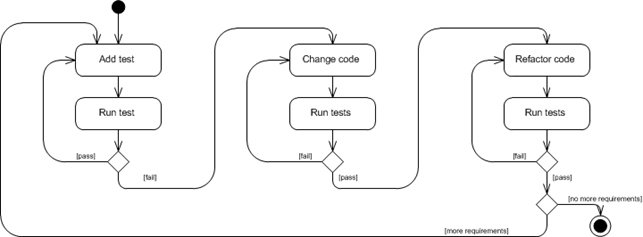
\includegraphics[width=\linewidth]{figs/tdd}
\caption{Red-Green-Refactor mamtra med TDD.}
\label{fig:tdd}
\end{figure}

\subsection{Feature list}
En \textit{feature list} indeholder (pudsigt nok) features, som ønskes implementeret. Herefter udvikler man bare én feature af gangen. \textit{Feature listen} skal indeholde en beskrivelse samt et sæt af test for den pågældende feature.

\subsection{Red-Green-Refactor}
Bruges til at beskrive selve arbejdsmetoden som anvendes ved TDD.

\begin{enumerate}
	\item Skriv en test som skal fejle\footnote{Hvis testen ikke fejler første gang, er der noget galt.}.
	\item Koden skrives så testen præcis bestås.
	\item Koden refaktueres.
\end{enumerate}

Fordelen ved dette skulle gerne være at man er tvunget til at skrive \textbf{blackbox-test}, at koden bliver meget testbar og unødvendig koden holdes på et minumum.

\begin{figure}[H]
\centering
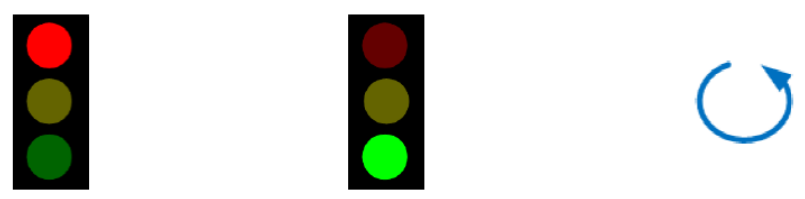
\includegraphics[width=0.7\linewidth]{figs/redgreen}
\caption{Red-Green-Refactor. Fejl, Implementer, refactor.}
\label{fig:redgreen}
\end{figure}

\subsection{Fordele og Ulemper}

\begin{itemize}
	
	\item \textbf{Fordele}	
	\begin{itemize}
		\item Koden bliver forklaret gennem test, jf. naming-convention.
		\item Man overvejer nødvendigheder i stedet for implementering.
		\item Koden bliver testbar og gennemtestet.
	\end{itemize}
	
	\item \textbf{Ulemper}	
	\begin{itemize}
		\item Forlænget udviklingstid - skulle gerne lede til besparet tid på vedligeholdelse mm.
		\item Kræver stor selvdisiplin - man skal ikke ''bare lige'' implementerer noget før det er nødvendigt.
	\end{itemize}
		
\end{itemize}
































